\documentclass[11pt, a4paper]{article}

% Configuración de márgenes de las páginas
\usepackage{a4wide}

% Paquete de acentos para Linux
\usepackage[utf8]{inputenc}

% Paquete de acentos para windows
%	\usepackage[latin1]{inputenc}

% Paquete para reconocer la separación en sílabas en español
\usepackage[spanish]{babel}

% Paquetes especiales para el TP
\usepackage{./otros/caratula}
\usepackage{./otros/algo2symb}
\usepackage{./otros/shortlst}
\usepackage[lined]{./otros/algorithm2e}
\usepackage{amssymb}			%simbolos matematicos
\usepackage{pdfpages}


% Paquete para incluir hypervinculos
\usepackage{color}
\usepackage{url}
\definecolor{lnk}{rgb}{0,0,0.4}
\usepackage[colorlinks=true,linkcolor=lnk,citecolor=blue,urlcolor=blue]{hyperref}

% Paquete para armar índices
\usepackage{makeidx}
\makeindex

% Más espacio entre líneas
\parskip=1.5pt

% Comandos personalizados
\newcommand{\nat}{\ensuremath{\mathbb{N}}}
\newcommand{\entero}{\ensuremath{\mathbb{Z}}}
\newcommand{\real}{\ensuremath{\mathbb{R}}}
\newcommand{\tab}{\hspace{1em}}

\begin{document}

% Carátula
\titulo{Trabajo Práctico Final}
\fecha{Marzo de 2010}
\materia{Organización del Computador II}
\integrante{Bianchi, Mariano}{92/08}{marianobianchi08@gmail.com}
\integrante{Brusco, Pablo}{527/08}{pablo.brusco@gmail.com}
\integrante{Di Pietro, Carlos Augusto Lyon}{126/08}{cdipietro@dc.uba.ar}
\maketitle

% Índice
\small
\newpage \printindex \tableofcontents
\normalsize
\newpage

% Cuerpo del informe
\section{Introducción}
	\paragraph{}
	El presente trabajo final surge como una continuación del tercer trabájo práctico de la materia en el segundo cuatrimestre de 2009. Aquél trabajo consistía en implementar un sistema minimal que permitiese correr concurrentemente dos tareas. Concretamente, dicho sistema consitía en un bootloader que se encargaba de cargar a memoria un kernel simplificado que incluía los binarios de las tareas en cuestión, junto con todas las estructuras necesarias para que dichas tareas pudieran ser ejecutadas (GDT, Directorio de Tablas de Páginas, una Tabla de Páginas para cada tarea, etc.). Luego, el kernel simplemente debía encargarse de activar el \textit{Gate A20}, pasar el procesador a modo protegido, activar el sistema de paginación, y poner a correr las tareas llamadas ``Pintor'' y ``Traductor'', las cuales alternaba mediante una interrupción del timer.

	\paragraph{}
	Por el contrario, el trabajo aquí presentado, si bien se basa en el anterior, posee algunas diferencias. A pesar que las tareas de usuario se encuentran cargadas en memoria de manera estática, el principal aspecto que diferencia al presente trabajo, es que estas se van inicializando a medida que el usuario así lo desee, a través del manejo de una consola diseñada para dicho fin. A la hora de inicializar una tarea, esta es puesta en ejecución a través de un scheduler que va asignando tiempos de CPU a cada uno de los procesos que se ejecutan de forma concurrente en el sistema. Naturalmente, esta diferencia en cuanto al otro kernel conlleva un cambio en lo que respecta a la administracíón de memoria, ya que estructuras como entradas de la GDT o TSS's deberán ser creados e inicializados para cada nueva tarea conforme estas van siendo lanzadas.\\
	En consecuencia, el resultado final es un \textit{kernel multitarea} (es decir capaz de ejecutar varias tareas alternadamente dando la ilusión de simultaneidad) que puede lanzar procesos de forma dinámica con tan solo cargar tareas de memoria y creando las estructuras necesarias para que estas puedan ejecutarse en un procesador de arquitectura Intel-x86.


\section{Instrucciones de uso}
	\paragraph{}
	Para ejecutar el kernel basta con compilar el kernel utilizando el MakeFile. Luego utilizando Bochs 2.4 se iniciara el proceso. Una vez cargado, el kernel mostrará en pantalla una consola mediante la cual se podrá cargar y poner a ejecutar cada una de las tareas. A continuación se detallan la lista de comandos que pueden ser interpretados por la consola:
	\begin{itemize}
		\item "h" : ayuda (lista los comandos).
		\item "l" : muestra todas las tareas disponibles.
		\item "p" : muestra todas las tareas en ejecuci\'on junto con su pid.
		\item "v \{x\}" : ejecuta y muestra la tarea \{x\}.
		\item "d \{pid\}" : muestra la tarea con pid \{pid\}.
		\item "k \{pid\}" : termina la tarea con pid \{pid\}.
	\end{itemize}


\section{Implementación}
\subsection{Descripción General}
	\paragraph{}
	El código fuente que implementa el kernel se entrega junto con este informe en un sorpote digital y se ubica en la carpeta \texttt{codigo}. Dentro de la misma los archivos se organizan de la siguiente manera:
	\begin{center}
		\begin{shortitemize}
		\setlength{\shortitemwidth}{200pt}
		\item Memoria
		\item Scheduler
		\item GDT - Global Descriptor Table
		\item Paginación				
		\item Consola
		\item Pantalla
		\item TSS - Task State
		\item BCP - Block Control Process
		\item Interrupciones							
		\item Kernel
		\end{shortitemize}
	\end{center}		

	\paragraph{}
	Esta distribución no es arbitraria, sino que responde a la modularización con la cual se encaró el diseño y desarrollo del kernel aquí presentado. Así, cada directorio contiene el código fuente de uno o más de los módulos que integran al kernel, cada uno de los cuales fue desarrollado de forma incremental y testeado individualmente.

	\paragraph{}
	En la sección \ref{modulos}, se procederá a explicar en detalle cada uno de estos módulos a fin de poder comprender con claridad todas las partes que componen al kernel elaborado. Una vez concluída esa explicación, en la sección siguiente (\ref{kernel}), se detallará de qué forma el kernel agrupa y hace uso de todos estos módulos a fin de dar como resultado un sistema \textit{multitasking} con un \textit{scheduler} dinámico capaz de levantar tareas de memoria y alternarlas por medio de una política de reemplazo \textit{Round Robin}.

	\paragraph{}
	Seguidamente, se expone cómo está constituído el \textit{Mapa de memoria} del sistema, así como también el porqué de su elección.


\subsection{Mapa de Memoria}
	\paragraph{}
	Previo a la escritura del código de los módulos mencionados en la sección anterior, a sabiendas de que el sistema utilizaría la paginación como forma de direccionar a memoria, se procedió a establecer un mapa de memoria que permitiese ubicar las estructuras críticas e indispensables del sistema de manera inequívoca. La opción elegida fue realizar un \textit{identity mapping} de las páginas (todas ellas de 4 KB) a los frames de memoria, fijando algunos de ellos para uso exclusivo del kernel o de otras estructuras como la \textit{GDT}, las \textit{TSS} o el \textit{Bitmap}.

	\paragraph{}
	La imagen que sigue muestrá como estan mapeadas y ocupadas las páginas de memoria en el sistema:
	\begin{center}
		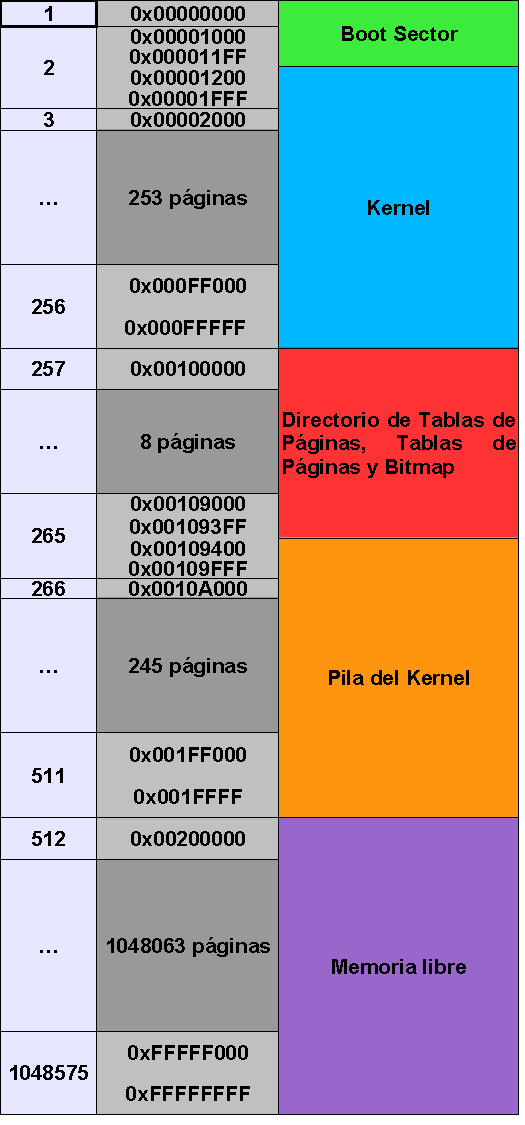
\includegraphics[scale=0.80]{./otros/mapa_memoria.pdf}
	\end{center}

\subsection{Módulos}
\label{modulos}
\subsubsection{Memoria}
\label{mem}
	\paragraph{}
	El módulo de \textbf{Memoria} es el encargado de brindarle al kernel las herramientas para contabilizar y administrar la memoria del sistema.

	\paragraph{}
	Básicamente, la idea empleada para administrar consiste en contabilizar la cantidad de bytes con los que cuenta la memoria, luego determinar cuántas páginas de 4 KB hay en la memoria del sistema y luego plasmar esta información en un \textit{Bitmap}. El \textit{Bitmap} no es más que una porción de memoria en donde hay tantos bits como páginas haya en el sistema. Luego, cada página ocupada se representa en el \textit{Bitmap} poniendo un ``1'' en el bit asociado a dicha página, mientras que las páginas libres se representan con un ``0''.

	\paragraph{}
	En líneas generales la interfaz de este módulo puede ser caracterizada de la siguiente manera:
	\begin{itemize}
		\item Variables Globales:
		\begin{itemize}
			\item \texttt{memoria\_total:} Variable global en la cual se almacena la cantidad de Megabytes de memoria con la que cuenta el sistema.
			\item \texttt{paginas\_libres:} Variable global que contabiliza el número de páginas libres de memoria en el sistema.
			\item \texttt{dir\_init\_bitmap:} Puntero a la dirección 0x???, que es la posición donde se inicia el \textit{Bitmap} para administrar las páginas de memoria.
			\item \texttt{dir\_end\_bitmap:} Puntero a la dirección 0x??, que es la última dirección válida del \textit{Bitmap}.
		\end{itemize}
		\item Funciones:
		\begin{itemize}
			\item \texttt{contarMemoria:} Función que se encarga de contar cuántos MB de memoria hay en el sistema guardando dicho valor en la variable \texttt{memoria\_total}. Asímismo, determina el número de frames de 4 KB que puede haber en la memoria del sistema y almacena dicho valor en la variable \texttt{paginas\_libres}.
			\item \texttt{llenarBitmap:} Función que a partir de la posición apuntada por \texttt{dir\_init\_bitmap} marca poniendo en ``1'' todos los bits correspondientes a las páginas de memoria utilizadas por el kernel y luego pone en ``0'' a las restantes.
			\item \texttt{pidoPagina:} Función que devuelve un puntero a la primer posición de memoria de una pagina libre, y previo a ello, la marca como ocupada en el Bitmap poniendo en ``1'' el bit correspondiente a dicha página.
			\item \texttt{liberoPagina:} Función que dado un puntero a una posicion de memoria, determina en qué página de memoria se alberga dicha posición y luego pone en ``0'' el bit correspondiente a esa página para así marcarla como libre.
			\item \texttt{setmem:} Función que dado un puntero a una posición de memoria y dos valores enteros \textit{set} y \textit{cant}, pone el valor de \textit{set} en \textit{cant} bytes desde la posición de memoria apuntada por el puntero en adelante.
			\item \texttt{cpmem:} Función que dados dos punteros a posiciones de memoria y un valor entero \textit{cant}, copia el valor de \textit{cant} bytes desde la posición de memoria apuntada por el primer puntero en adelante, hacia los \textit{cant} bytes de memoria desde la posición de memoria apuntada por el por el segundo puntero en adelante.
		\end{itemize}
	\end{itemize}

\subsubsection{Global Descriptor Table (GDT)}
\label{gdt}
	\paragraph{}
	El módulo de \textbf{GDT} es aquel mediante el cual se introduce la estrutura de datos \textit{GDT} que modela la estructura \textit{Global Descriptor Table} de la arquitectura IA-32 de Intel\footnote{Intel 64 and IA-32 Architectures Software Developer’s Manual, Volume 3A: System Programming Guide, Part 1 - Sección 2.1.1, página 61}. Asímismo, implementa también las funcionalidades necesarias para que el kernel pueda operar y hacer uso de esta estructura.

	\paragraph{}
	Concretamente, la implementación de la estructura \textit{GDT} no es más que un arreglo de otra estructura más pequeña definida en este mismo módulo: la \textit{GDT\_entry}. Dicha estructura constituye un bloque de memoria de 4 bytes que modela las entradas en la \textit{GDT}, las cuales reciben el nombre de descriptores. Los descriptores pueden ser de varios tipos (descriptor de segmento, descriptor de TSS, etc) y se separan en diversos campos. Por tal motivo, la estructura \textit{GDT\_entry} también está subdividida en idénticos campos los cuales, segun los valores que se le fijen, indican entre otras cosas a qué tipo de descriptor corresponde cada entrada.

	\paragraph{}
	Finalmente, nuestra GDT queda organizada de la siguiente manera:

	\begin{itemize}
		\item entrada nula
		\item codigo kernel
		\item datos kernel
		\item codigo usuario
		\item datos usuario
		\item descriptor\_tss1
		\item descriptor\_tss2
		\item ...	
		\item descriptor\_tssx
	\end{itemize}

	\paragraph{}
	En el módulo implementado podemos encontrar las siguientes funciones:

	\begin{itemize}
		\item \texttt{make\_descriptor}: función que crea una entrada para la gdt tomando como parametros la base, el limite y los atributos.
		\item \texttt{buscar\_entradaGDT\_vacia}: Devuelve una posicion de la gdt que este vacia.
		\item \texttt{borrar\_gdt\_entry}: Crea un descriptor vacio en la posición a borrar.
	\end{itemize}

\subsubsection{Paginación}
\label{pag}
	\paragraph{}
	En este módulo, podemos encontrar todas las funcionalidades necesarias para el manejo de la paginación, las cuales son:
	
	\begin{itemize}
		\item mapear\_tabla
		\item mapear\_pagina
		\item obtener\_mapeo
		\item iniciar\_paginacion\_kernel
		\item liberar\_directorio
	\end{itemize}

	\paragraph{}
	Cuando se hizo necesario implementar el módulo, nos dimos a la tarea de imaginar qué necesidades íbamos a tener respecto a la paginación. En un comienzo, las rutinas \textit{mapear\_tabla} y \textit{mapear\_página} eran precarias. Necesitaban recibir como parámetro la dirección de la entrada de directorio y la de tabla de páginas respectivamente. Esto resultaba molesto, ya que primero habia que hacer un cálculo para conocer el offset dentro de cada tabla antes de poder realizar el mapeo. Además, en el caso del mapeo de una página, también habia que verificar que la tabla de páginas asociada a la página que se intentaba mapear estuviera presente.

	\paragraph{}
	Teniendo en cuenta estas desventajas, se concluyó que era necesario que todos estos cálculos y verificaciones se hicieran dentro de las mismas funciones. Seguidamente, se modificó el código de \textit{mapear\_página} para que sólo reciba la dirección fisica del directorio de páginas, además de las necesarias como dirección virtual (o lógica), dirección física a la cual se debía mapear la dirección virtual y los atributos de dicha página (escritura/lectura, supervisor/usuario, presente/no presente). Una de las principales características de la función es que allí se hace la verificación de si está o no presente la tabla de páginas que corresponde, y en caso de no estarlo, se pide una página para su estructura, se la inicia usando \textit{mapear\_tabla} y luego se continúa con el mapeo deseado. Estas características hicieron mucho más simple su uso y nos facilitó la tarea a la hora de programar otras rutinas que dependían de esta implementación.

	\paragraph{}
	Por otra parte, está la función \textit{iniciar\_paginacion\_kernel}, que simplemente inicializa el Directorio de Tablas de Páginas (DTP) y todas las Tablas de Páginas (TP) asociadas. Para ello, se reservó una dirección dentro del mapa de memoria (la dirección es 0x100000), en la cuál se alojan todas estas estructuras.

	\paragraph{}
	La última función crucial de este módulo es \textit{liberar\_directorio}. Esta función se encarga de, dada la dirección de un directorio de tablas de páginas, borrar todas las entradas del directorio y de las tablas de páginas y limpiar y liberar todas aquellas páginas que hayan sido utilizadas para contener estas estructuras, las páginas de las pilas de la tarea y del buffer de video. Esta función es utilizada a la hora de eliminar una tarea de memoria.

\subsubsection{TSS}
\label{tss}
	\paragraph{}
	La TSS (Task State Segment) es una estructura de datos que contiene informaci\'on acerca de una tarea. 

	\paragraph{}
	Para setear la TSS se necesita una entrada en la GDT especificando la base, limite y atributos.

	\paragraph{}
	Luego, para acceder al c\'odigo de la tarea, deberemos, entre otras cosas, hacer un jump al descriptor de TSS en la gdt.

	\paragraph{}
	En nuestro kernel, las funciones que poseemos en este módulo son:
	\begin{itemize}
		\item \texttt{crear\_TSS}: Crea una TSS (y su descriptor en la GDT) utilizando como parametros: dirección, CR3, EIP, EFLAGS, pila y el ESP0.
		\item \texttt{buscar\_TSS\_vacia}: Busca una entrada de TSS vacia (toma como TSS vacia aquella cuyo cr3 sea igual a 0, devuelve un número igual o mayor que CANT\_TAREAS si no hay ningun lugar disponible)
		\item \texttt{vaciar\_TSS} Setea el cr3 de una tss en 0 para ser reutilizada por otras tareas.
	\end{itemize}

\subsubsection{Process Control Block (BCP) }
\label{bcp}
	\paragraph{}
	El Process Control Block, es una estructructura de datos en el Kernel que contiene la información necesaria para manejar cada uno de los procesos.
	En nuestro caso, esta estructura contiene la siguiente información:
	\begin{itemize}
		\item \textbf{pid}: indice de la tarea en el gdt\_vector
		\item \textbf{estado}: indica el estado de la tarea
		\item \textbf{entrada\_directorio}: direccion del directorio de la tarea
		\item \textbf{sig}: siguiente tarea para el round robin scheduler
		\item \textbf{ant}: anterior tarea para el round robin scheduler
		\item \textbf{pantalla}: puntero a la pagina destinada al video de la tarea
		\item \textbf{nombre}
		\item \textbf{dir\_fisica}: puntero a la/s página/s a donde fue copiada la tarea para ejecutarse
	\end{itemize}

	\paragraph{}
	Ya que el BCP contiene informacion critica de los procesos, esta almacenada en un area protegida de los usuarios. En nuestro caso la protección que tiene es la misma que la de todo el kernel. El usuario tiene permisos de lectura, pero no de escritura.

	\paragraph{}
	Las principales funciones del módulo BCP son las siguientes:

	\begin{itemize}
		\item \texttt{iniciar\_BCP}: llena el BPC[0] con los datos del kernel, y inicializa variables globales
		\item \texttt{buscar\_entradaBCP\_vacia }: busca entrada libre en el BCP (libre significa estado muerto)
		\item \texttt{crear\_entradaBCP }: llena la entrada con los datos de la tarea y la agrega al final de la cola de tareas activas
		\item \texttt{cambiar\_estado}: cambia el estado de una tarea, y si el estado es MUERTO la quita de la cola de tareas activas
		\item \texttt{buscar\_entradaBCP}: devuelve la posicion en la BCP de una tarea pasada como parametro.
		\item \texttt{buscar\_entradaBCP\_matar}: devuelve la posicion en la BCP de alguna tarea con estado "MUERTA". Si no hay ninguna, devuelve CANT\_TAREAS
		\item \texttt{cargarTarea}: carga una tarea y todo sus datos y contexto en memoria y la agrega en la BCP para incluirla en el scheduling
		\item \texttt{matarTarea}: Marcar tarea como "MATAR" para que luego el KERNEL se encargue de eliminarla. 
		\item \texttt{exit}:  esta es llamada cuando la tarea actual quiere terminar y llama a la interrupcion 80
		\item \texttt{desaparecerTarea}: Esta funcion se va a llamar cada vez que se ejecute el kernel. La idea es que si hay alguna tarea en la BCP marcada como "MATAR" (ya va a estar fuera del scheduler), esta funcion se encargue de eliminar y liberar todas las estructuras utilizadas por la tarea (BCP, TSS, directorio y tablas de páginas, paginas de video y de pila y gdt).
	\end{itemize}

\subsubsection{Interrupciones}
\label{int}
	\paragraph{}
	Las estructuras y funciones necesarias para el manejo de interrupciones en el kernel aquí presentado se encuentran implmentadas en dos módulos: 
	\begin{itemize}
		\item El primero se encarga de la creación y el manejo de las estructuras necesarias para el funcionamiento de las interrupciones: \textit{IDT, descritores de IDT, registro de IDT, etc}.
		\item El segundo se encarga de definir cada una de las funciones que constituyen las rutinas de atencion de interrupciones.
	\end{itemize}
	
	\paragraph{}
	El primer módulo está compuesto por los archivos \textit{idt.c} e \textit{idt.h}. Allí se especifican las estructuras \textit{IDT} e \textit{IDT\_Descriptor} que modelan respectivamente la \textit{Interruption Descriptor Table (IDT)} y el \textit{registro de GDT (GDTR)} de la arquitectura IA-32 de Intel\footnote{Intel 64 and IA-32 Architectures Software Developer’s Manual, Volume 3A: System Programming Guide, Part 1 - Sección 6.10, página 226}.\\
	Al igual que la estructura \textit{GDT} descripta en la sección \ref{gdt}, la \textit{IDT} es un arreglo de otra estructura menor que es la \textit{IDT\_entry}, la cual a su vez modela las entradas de la \textit{IDT} que reciben el nombre  de \textit{descriptores de IDT}\footnote{Intel 64 and IA-32 Architectures Software Developer’s Manual, Volume 3A: System Programming Guide, Part 1 - Sección 6.11, página 228}.
	
	\paragraph{}
	A continuación presentamos la interfaz de este módulo explicando cada una de las funciones que brinda al kernel para el manejo de las estructuras antes explicadas:
	\begin{itemize}
		\item \texttt{set\_interrupt:} Setea una \textit{IDT\_entry} con los valores necesarios para que sea un descriptor de interrupción.
		\item \texttt{set\_trap:} Setea una \textit{IDT\_entry} con los valores necesarios para que sea una trap gate.
		\item \texttt{set\_task\_gate:}  Setea una \textit{IDT\_entry} con los valores necesarios para que sea una puerta de tarea.
		\item \texttt{idtFill:} Setea las primeras 20 entradas de la \textit{IDT} como descriptores de interrupciones apuntando cada uno a su correpondiente rutina de atención, cada una de las cuales llama a su vez a la función \textit{handler\_de\_interrupciones}.	Luego, setea la entrada 32 y 33 de la \textit{IDT} como descriptores de interrupciones para el timertick y teclado respectivamente. Finalmente, setea la entrada 80 de la \textit{IDT} como un descriptor de interrupción que implementa la syscall \textit{exit} para matar al proceso que se encuentra en ejecución.
		\item \texttt{handler\_de\_interrupciones:} Esta función es llamada por las primeras 20 rutinas de atención de interrupciones para imprimir por pantalla el número de interrupción producido y colgar la ejecución del sistema.
	\end{itemize}
	
	\paragraph{}
	El segundo módulo es aque en el que se implementan las funciones \textit{\_INT\texttt{X}}, donde \texttt{X} el número de la interrupcion que al producirse invoca a su correspondiente función \textit{\_INT\texttt{X}}.
	
	\paragraph{}
	Seguidamente se expone la lista de rutinas de interrupción implementadas junto con una breve descripión de su funcionamiento:
	\begin{itemize}
		\item \texttt{\_INT0 a \_INT19:} Llama a la función \texttt{handler\_de\_interrupciones} pasándole como parámetro el número de la interrupción producida para que ésta imprima por pantalla un mensaje asociado a dicha interrupción y luego ejecute un loop infinito a fin de colgar la ejecución del sistema.
		\item \texttt{\_INT32:} Llama a la función \texttt{switch\_task} del módulo \textbf{Scheduler} para que se produzca el cambio de la tarea que se esta ejecutando por la tarea elegida por el \textit{scheduler} segun su politica de reemplazo.
		\item \texttt{\_INT33:} Copia el valor de la tecla pulsada en el registro \textit{AX} y llama a la función \texttt{console} (implementada en el módulo \textbf{Consola}) pasandole el valor de ese registro como parámetro.
		\item \texttt{\_INT80:} Llama a la función \texttt{exit} del módulo \textbf{BCP} que se encarga de imprimir en pantalla el mensaje \textit{``TERMINE!!''}, matar a la tarea que se está ejecutando y llamar a la función \texttt{switch\_task} para pasar a la proxima tarea segun la política de scheduling. 
	\end{itemize}

\subsubsection{Scheduler}
\label{sched}	
	\paragraph{}
	El algoritmo de scheduling es el que determina cuanto tiempo de CPU sera dedicado a cada proceso dependiendo cumpliendo con ciertos criterios
	\begin{itemize}
		\item todas las tareas deben poseer tiempo en la CPU.
		\item si se usan priordades, una tarea con menor prioridad no debería trabar a una de mayor prioridad.
		\item el scheduller debe escalar bien a medida que se agregan tareas en el kernel.
	\end{itemize}

	\paragraph{}
	Para este trabajo elegimos el algoritmo de Round Robin.

	\paragraph{}
	Este algorimo es simple ya que se utiliza una única cola de procesos. Cuando el tiempo de cada uno de estos pasa, se efectua un cambio hacia la ejecución del siguiente y el anterior es puesto nuevamente en la cola. 

	\paragraph{}
	Cada proceso posee un quantum (cierto numero de ticks del reloj) que es el tiempo en el que se estara ejecutando. En nuestro caso, cada quantum equivale a 1 tick de reloj.

	\paragraph{}
	En nuestro kernel, el scheduller esta compuesto por la funci\'on switch\_task, cuyo funcionamiento es el siguiente

	\begin{enumerate}
		\item comprueba que haya mas de una tarea, sino no hace nada.
		\item cambia el estado de la tarea actual de CORRIENDO a ACTIVO (o lo deja en MATAR si es que estaba asi)
		\item cambia el selector de 'salto' a donde se marco el 'pid' de la tarea\_actual, teniendo en cuenta qué RPL (Requested Privileged Level) elegir dependiendo de qué tarea se va a pasar a ejecutar
		\item se hace el cambio de tarea
	\end{enumerate}


\subsubsection{Consola}
\label{cons}
	\paragraph{}
	La consola es una función del kernel que permite una interfaz hacia los usuarios, en este caso es una linea de comandos que permite listar, correr, matar, etc. una lista de tareas disponibles en el sistema. 

	\paragraph{}
	A continuación se listan las principales funciones necesarias para hacer posibles la linea de comandos:
	\begin{itemize}
		\item \texttt{ cargar\_tarea}: recibe la posicion de la tarea a cargar dentro de "tareas\_en\_memoria"
		\item \texttt{console}: Es la función llamada cada vez que se preciona una tecla en la linea de comandos. En caso que esta tecla sea un 'enter' se llama a la función 'run' del comando almacenado, en caso contrario se van almacenando las teclas.
		\item \texttt{run}: Es la encargada de obtener y decodificar el comando enviado por console de manera de llamar a la función correcta.
	\end{itemize}				


\subsubsection{Pantalla}
\label{screen}
	\paragraph{}
	El módulo pantalla se ocupa de lo necesario para poder imprimir información en la pantalla para el uso del kernel y las tareas.

	\paragraph{}
	Está planeado de la siguiente manera:
	\begin{itemize}
		\item 23 filas centrales que podras usar las tareas y el kernel para escribir
		\item En la última fila se vera la linea de comandos (manejada por console.c) 
	\end{itemize}
	 
	\paragraph{}
	Las funciones que provee son:
	\begin{itemize} 
		\item \textbf{avanzar\_puntero}: Avanza el puntero de la pantalla un caracter. 
		\item \textbf{retroceder\_puntero}: Retrocede el puntero de la pantalla un caracter. 
		\item \textbf{mover\_puntero}: Mueve el puntero de la pantalla hasta una fila y columna indicadas. 
		\item \textbf{salto\_de\_linea}: Avanza el puntero de la pantalla una fila. 
		\item \textbf{printf}: Es utilizadad para imprimir caracteres.
		\item \textbf{printdword}: Se usa para ver valores de variables. Recibe como parámetros la dword a imprimir y los atributos de escritura.
		\item \textbf{putc}: Escribe un caracter en la pantalla 
		\item \textbf{borrarc}: Borra el ultimo caracter de la pantalla 
		\item \textbf{num2char}: Deja en buffer un string que representa al numero pasado escrito en una base indicada. 
		\item \textbf{clear\_screen}: Limpia la pantalla. 
		\item \textbf{mostrar\_pantalla\_entera}: La idea es copiar 23 renglones enteros de la tarea 'pid'. (Recordar que la pantalla es de 80*23, de manera de dejarle el ultimo 'renglon' para el kernel y la consola y el primer renglón para saber qué estamos visualizando.
		\item \textbf{cambiar\_pantalla}: Setea la pantalla a mostrar y llama a mostrar pantalla entera.
		\item \textbf{clear\_command\_line}: limpia la linea de comandos (fila 24 de la pantalla) y deja el prompt y el puntero a dicha linea inicializado 
		\item \textbf{clear\_info\_line}: Limpia la linea de informacion (fila 0 de la pantalla) y deja el puntero a dicha linea inicializado 
		\item \textbf{removerc}: Borra el ultimo caracter de la linea de comandos 
		\item \textbf{agregarc}: Escribe un caracter en la linea de comandos
	\end{itemize}


\subsection{El Kernel}
\label{kernel}	
	\paragraph{}
	Hasta aquí se explico el funcionamiento de todos los módulos que componen el kernel. En esta sección, se explicará cómo se integran todos estos componentes para conformar el kernel propiamente dicho. Veamos entonces cómo se conforma el módulo \textbf{Kernel}.
	
	\paragraph{} 
	Los archivos del módulo \textbf{Kernel} son tres: \textit{kernel.c}, \textit{kernel.h} y \textit{kernel.asm}. Los dos primeros, son archivos que contienen la declaración e implementación de funciones que serán utilizadas por el kernel durante su ejecución. Estas son:
	\begin{itemize}
		\item \texttt{kernel\_infinito:} Esta función consistuye el loop infinito sobre el cual se basa todo kernel. Durante este ciclo, la única acción del kernel consiste en la búsqueda de algún proceso al que se lo haya marcado en su entrada de \textit{BCP} como listo para matar y se procede a la liberación de todos los recursos asociados a ese procesos (páginas de memoria, TSS, pila, entrada en la \textit{BCP}, entrada en la \textit{GDT}).
		\item \texttt{update\_cursor:} Esta función únicamente se encarga de mover el cursor que está en la pantalla.
	\end{itemize}
	
	\paragraph{}
	Finalmente, el archivo \textit{kernel.asm} contiene el código de inicialización del kernel, que es en donde finalmente se hace uso de todas de las estructuras y funcionalidades aportadas por los módulos vistos anteriormente. A continuación, se detallará todos los pasos que realiza el kernel a fin de preparar el sistema para que sea capaz de ejecutar tareas de modo concurrente, para luego, mediante la invocación a la función \texttt{kernel\_infinito}, dar paso a la posible ejecución de las mismas:
	
	\begin{enumerate}
		\item Como primer paso, se habilita el Gate A20 para que se pueda direcciónar a memoria más alla de la dirección 0x100000; es decir, más allá de 1 Megabyte.
		\item Luego, se carga la estructura \textit{GDT\_desc} del módulo \textbf{GDT} en el registro \textit{gdtr} del procesador, el cual describe la direción base y el límite de la \textit{GDT}. A su vez, la \textit{GDT}, que tal como se explicó oportunamente en la sección \ref{gdt} es un arreglo de descriptores, también es inicializada seteando la memoria contigua al código del kernel (hacia el final del archivo \textit{kernel.asm}) de forma tal que allí queden alojados los 128 descriptores detallados en la sección \ref{gdt}. 
		\item Seguidamente se setea el bit \textit{PE} de registro \textit{CR0} del procesador a fin de poder realizar el pasaje a \textit{modo protegido}.
		\item Luego se ejecuta la instrucción \texttt{Jmp 0x08:modo\_protegido} a fin de efectivizar el pasaje al \textit{modo protegido} del procesador. Asímismo, se actualiza el valor de los registros selectores para que apunten al descriptor de segmento de datos en la \textit{GDT}.
		\item A continuación, se inicializa la pila en la posición de memoria 0x200000 (2 MB) guardando este valor en los registros \textit{ESP} y \textit{EBP} del procesador. Se asume que el sistema cuenta con esa mínima cantidad de memoria, ya que es requerimiento para la correcta ejecución del kernel.
		\item Una vez hecho esto se realiza un llamado a la función \texttt{contarMemoria} del módulo \textbf{Memoria} a fin de poder inicializar las variables \texttt{memoria\_tota, paginas\_libres} con valores acordes a la memoria del sistema sobre el cual se está ejecutando el kernel.
		\item Luego, se hace una invocación a la función \texttt{iniciar\_paginacion\_kernel} del módulo \textbf{Paginación} para setear e inicializar las estructuras necesarias (directorios, tablas de páginas, páginas) a fin de que el sistema pueda trabajar con este método de direccionamiento a memoria.
		\item Inmediatamente después se procede a cargar el registro \textit{CR3} del procesador con la direccion del \textit{Directorio de Tablas de Páginas} para que el procesador pueda ubicar esta estructura en memoria al momento de convertir las direcciones lógicas a direcciónes físicas.
		\item Seguidamente, se habilita la unidad de paginación en el procesador. Para ello, se setea el bit \textit{PG} del registro \textit{CR0}.
		\item Luego, una vez habilitada la paginación, se invoca a la función \texttt{llenarBitmap} del módulo \textbf{Memoria} para marcar como ocupadas a todas las páginas utilizadas por el kernel y como libres a las restantes. De este modo, el kernel ya tiene control y puede administrar la memoria del sistema.
		\item A continuación se llama al a función \texttt{iniciar\_BCP} del módulo \textbf{BCP}. De esta forma, se inicializan las variables globales relativas a los procesos y se marca al kernel como el ``proceso 0'', llenando la primera entrada la \textit{BCP} con los datos del mismo. Esto posibilitará que cuando el kernel esté corriendo su loop infinito y haya más tareas en el sistema sea ``scheduleado'' como una tarea más, pudiendo retomar el control del procesador únicamente cuando el scheduler le de su turno.
		\item Sabiendo que las tareas se alternarán el control procesador, es preciso conservar el entorno de ejecución del kernel para cuando éste retome el control del mismo. Para ello, en este punto de la inicializacion se llama a la función \texttt{iniciar\_tss\_kernel} del módulo \textbf{BCP} que se encarga de buscar una \textit{TSS} en el arreglos de \textit{TSS's}, guardar el contexto de ejecución en la misma y colocar el corespondiente descriptor de \textit{TSS} en la \textit{GDT}.
		\item Luego, se carga el registro de tareas (\textit{TR}) del procesador \textbf{.... ???}
		\item Finalmente, solo resta inicializar todo lo referente a las interrupciones el sistema. Con tal propósito se llama a la función \texttt{idtFill} del módulo \textbf{Interrupciones} para que defina la correspondiente rutina de atención a cada una de las posibles interrupciones.
		\item Seguidamente, se procede a remapear las interrupciones del vector de interrupciones \textbf{.... ???}
		\item Luego, se carga el valor la estructura \textit{IDT\_Descriptor} declarada en el módulo de \textbf{Interrupciones} dentro del registro \textit{IDTR} del procesador para indicarle a éste cuál es la direccion base y el limite de la \textit{IDT}.
		\item Como paso siguiente, se habilitan las interrupciones en el sistema mediante la instrucción en assembler \texttt{sti}. 
		\item Y finalmente, se invoca a la función \texttt{kernel\_infinito} del módulo \textbf{Kernel} para lograr de esta forma un loop infinito, en el cual además se buscan procesos finalizados y se liberan sus recursos.
	\end{enumerate}

	\paragraph{}
	Una vez finalizada la inicialización del kernel, el sistema cuenta con todas las estructuras necesarias y queda listo para que por medio de la consola el usuario ponga a correr una o más tareas.
	
	\paragraph{}
	En la sección que sigue, se procederá a explicar qué ocurre en el sistema y qué operaciones tienen lugar desde que se carga una tarea nueva en el sistema hasta que la mismas es terminada.

\section{Cómo funciona todo}
\subsection{Introducción}
	\paragraph{}
	En las secciones anteriores de este informe se realizó una explicación a grandes rasgos de todas las estructuras y métodos utilizados para la implementación, inicialización y puesta en ejecución de un kernel multitasking. En la presente sección, se expondrá de qué forma las tareas son puestas en ejecución, alternadas entre sí y finalmente finalizadas.
	
	\paragraph{}
	Con este propósito, y a fin de entender más claramente cómo es la dinamica y el funcionamiento del sistema en cuanto al manejo de tareas, creemos que sería de mucha ayuda hacer una descripción paso a paso de algún posible escenario.

	\subsection{Escenario}
	\paragraph{}
	Describiremos entonces qué ocurre en el kernel cuando un usuario pone a correr dos tareas (que eventualmente pueden ser la misma) y luego decide finalizar una. Para ello, explicaremos paso por paso los eventos y acciones que tienen lugar en el sistema en el marco de la situación presentada:
	\begin{enumerate}
		\item Se inicia el sistema. Se ejecuta la inicilización del kernel tal como fue descripta en la sección  \ref{kernel}. Una vez terminada, la ejecución queda atrapada en el loop infinito de la función \texttt{kernel\_infinito}. No obstante, como las interrupciones están activas, el \textit{timertick} interrumpe al procesador cada \textbf{?? ms}.\\
		Una vez producida una interrupción del timer, se detiene la ejecución del loop y se pasa a ejecutar la rutina de atención de la interrupcion del timer (\#32) sin que se produzca ningún cambio de contexto; es decir, se guarda el \textit{instruction pointer (IP)} actual en la pila de la tarea que se esta ejecutando (que casualmente es el kernel) y se actualiza el valor del \textit{IP} a la dirección de memoria en donde está el código de la rutina \texttt{\_INT32}. Dicha rutina efectua un llamado a la función \texttt{switch\_task} del módulo \textbf{Scheduler}. Sin embargo, como no hay otras tareas en el sistema, la misma no realiza cambio alguno por lo que la interrupcion finaliza y el loop infinito de \texttt{kernel\_infinito} continúa su ejecución.\\
		Esta situación se repite continuamente y de forma indefinida hasta que el usuario ingrese algun comando por consola.
		\item Una vez que esto ocurre ...
		\item Se carga la tarea 1.
		\item El usuario ingres un comando para cargar una segunda tarea.
		\item Se carga la tarea 2.
		\item El usuario ingresa un comando para finalizar la primera tarea.
		\item Se elimina la tarea 1.
	\end{enumerate}


\section{Nosotros también nos equivocamos}
	\paragraph{}
	A lo largo de la realización del trabajo práctico fuimos encontrándonos con infinidad de problemas. Muchos fueron fáciles de descubrir y resolver, pero con otros no se contó con la misma suerte. Muchas veces estuvimos trabados mucho tiempo hasta poder continuar programando ya que había errores que no nos dejaban seguir adelante. Por esta razón es que creemos que en este informe no podía faltar una sección comentando alguno de los errores que nos causaron mayores dolores de cabeza.

	\paragraph{}
	Lo primero que se hizo a la hora de comenzar este trabajo práctico, fue limpiar el trabajo hecho en clase y sólo tomar las cosas básicas y primordiales, como la activación del GATE A20, la estructura de la GDT para el kernel, el paso a modo protegido y la actualización de los registros de segmento para que utilizaran los segmentos de la GDT correspondientes. Luego, comenzamos a trabajar en el resto de las funcionalidades, como la paginación, el manejo de memoria, etc. La idea era utilizar la menor cantidad de código assembler posible, para que el código resulte más legible y amigable, por lo tanto todas estas rutinas fueron implementadas en lenguaje C. Gracias a esta decisión, nos topamos con el primer problema. Intentando probar un código de C, durante el llamado a la función ocurría una excepción y la maquina virtual Bochs se colgaba. Intentando buscar donde estaba el error, fuimos comentando lineas de código de la función, hasta que finalmente se había comentado todo el código y sin embargo seguía ocurriendo la misma excepción. Lo que restaba entonces era que había un problema cuando se realizaba el llamado a dicha función. En ese momento, fue cuando caímos en la cuenta que nunca se había inicializado la pila del kernel. Asombrosamente, este error fue arrastrado desde el trabajo práctico realizado durante el cuatrimestre, pero en ese momento no había surgido este problema. La solución entonces fue cargar los registros \textit{EBP} y \textit{ESP} con la dirección destinada a la pila del kernel.

	\paragraph{}
	Más adelante, una vez que la cantidad de código había aumentado, nos topamos con otro error. Pero este error era distinto por una simple razón: el error se daba al compilar el kernel. En un comienzo no se entendía el por qué del problema. Luego de insistir un poco, pudimos entender a qué se debía. Dentro del código de error que nos daba al compilar, logramos ver que había algún problema con una variable llamada \textit{GDT\_DESC}. Esta variable pertenecía al código C de la GDT, y era la que contenía el tamaño y la dirección de la GDT. Notamos que este error dejaba de ocurrir si borrabamos o comentabamos líneas de código o eliminabamos alguna estructura de datos grande. Hecho esto, pudimos compilar y correr el código para poder debuggear. Lo primero que chequeamos fue la dirección en la que se alojaba dicha variable, la cuál rondaba por 0xFFxx (no registramos exactamente el valor para este apartado, pero estaba muy cerca de 0xFFFF). Revisando en qué parte del código se utilizaba esta variable, se notó que la misma sólo se usaba en las primeras líneas de código para cargar la GDT y poder así pasar luego a modo protegido. En este momento, recordamos que esas líneas de código utilizan el procesador en modo real, por lo que el código era procesado en 16 bits. Lo que ocurría entonces es que la dirección de la variable \textit{GDT\_DESC}, había superado la 0xFFFF y dicha dirección no era alcanzable por el código de 16 bits. Como no logramos encontrar la forma de indicarle al compilador GCC dónde queríamos que compilara cierto código, la solución que adoptamos fue implementar el arreglo de la GDT en assembler, dentro del archivo \textit{kernel.asm}. De esta manera nos aseguramos que el mismo quede en posiciones bajas de la memoria para que este error no volviera a ocurrir.

	\paragraph{}
	Una vez adentrados en la construcción del kernel, se optó por probar si se podía correr alguna tarea junto con el kernel utilizando todo lo que se había implementado hasta el momento, que si bien había sido probado por separado nunca se había puesto a prueba en una situación un poco más real. Lo primero que se intentó fue correr una tarea que se ejecutara en modo kernel es decir, igual a lo que se había realizado durante la cursada. En este caso no hubo inconveniente. Sin embargo, sí lo hubo al intentar correr una tarea en modo usuario. En este caso, cuando se intentaba realizar el switch de tareas, se producía una excepción de protección general (\#GP). Luego de ahondar un poco en el tema y de realizar algunas consultas a Alejandro Furfaro y a Federico Raimondo, pudimos resolver el problema modificando el RPL del selector con el cuál se hacían los cambios de contexto, es decir cuando se ejecutaba la instrucción \textit{jmp selector:offset}.

	\paragraph{}
	Sin embargo, este problema no terminó allí. Al momento de pasar a ejecutarse una tarea, sucedió que se producía un \textit{page fault}. Luego de hacer algunos debuggeos, notamos que este error se producía cuando la tarea intentaba escribir un dato en la pantalla. Estabamos seguros que el problema era de permisos, pero no lográbamos encontrar en dónde estaba. Luego de una nueva consulta, caímos en la cuenta que el error estaba en el permiso de la tabla de páginas. Cuando se había implementado la función mapear página, una de las verificaciones que se realizaba era para ver si la tabla de páginas estaba presente o no. Si no estaba, se alojaba una nueva página para la misma y se la mapeaba dentro del directorio de páginas en la entrada correspondiente, utilizando los mismos atributos/permisos que se usaban para la página que se estaba mapeando. El problema fue que el primer mapeo que se realizaba tenía permisos de lectura únicamente. Por lo que para la tabla de páginas que se utilizaba, sólo podían realizarse lecturas. Para corregir este error entonces, se procedió a modificar levemente el código de la función \textit{mapear\_pagina} verificando si el permiso de la página es de escritura y el de la tabla no, en cuyo caso se modificaban los permisos de la tabla de páginas. De esta manera, siempre prevalece el permiso más alto.

	\paragraph{}
	Uno de los problemas graves que nos surgieron a la hora del manejo de tareas fue cuando intentamos eliminar una tarea del scheduling. La idea principal era poder hacerlo a través de una llamada al sistema, pero sin embargo el primer objetivo fue lograr hacerlo desde alguna función que se pudiese llamar utilizando la consola. Algo así como el ``kill'' del sistema GNU/Linux (un poco más humilde en realidad). El primer problema que surgió fue que en algunas ocasiones funcionaba bien y en otras mal. La excepción que se producía era un \textit{page fault}. Luego de varios debuggeos, observamos que este error se producía cuando se estaba ejecutando la tarea a matar. Claramente, esto sucedía porque dentro de todas las acciones a realizar para eliminar a la tarea, una de ellas era vaciar (dejar en 0) el directorio de tablas de páginas. Claramente, estas posiciones de memoria no estaban dentro del mapeo de la tarea, por cuestiones de seguridad, además de no ser necesario en absoluto. Había varias soluciones distintas posibles de implementar, pero elegimos una que a los fines prácticos era más sencilla y que al igual que las otras, cumplía con los requisitos necesarios. Lo que se hizo entonces fue que el ``matar'' de una tarea fuese simplemente quitar a la tarea del scheduling modificando los punteros de las tareas que estaban alrededor de la tarea a matar y marcarla dentro de la BCP como tarea a matar. Luego, se agregó dentro del código del kernel que se buscara a las tareas a matar y que en caso de haberlas, ejecute ahora sí el código que se encargaba de limpiar y desocupar todas las estructuras utilizadas para dicha tarea (pilas, directorio y tablas, BCP, TSS, GDT, etc). Como esto se ejecutaba en el contexto del kernel, al tener el kernel toda la memoria mapeada en el directorio, quitamos el problema de los permisos a la hora de la limpieza. 

	\paragraph{}
	Luego de esta modificación, pudimos encontrar un problema que estábamos acarreando en una rutina de atención de interrupciones. Cuando corriamos el kernel, luego de un tiempo de inactividad, recibíamos una excepción \#GP. Luego de mucho debuggear, notamos que lo que ocurría es que se estaba realizando una llamada a la función que realizaba la limpieza de una tarea a pesar que en ningún momento se le había indicado. Más aún, ni siquiera se había cargado una tarea. Lo que ocurría es lo siguiente: en la ejecución del kernel, se realizaban 2 pasos:
	\begin{itemize}
		\item Se llama a una función que busca una tarea marcada como ``a matar'' dentro de la BCP
		\item Si el resultado de esta búsqueda es positivo (es decir, si hay alguna tarea así marcada), se llama a la función que limpia el contexto de una tarea.
	\end{itemize}

	\paragraph{}
	El problema fue que al parecer, esta función estaba retornando un valor erróneo. Sin necesidad de realizar un debbugeo, se descartó esta posibilidad porque el código de la esta función era muy simple y fácil de revisar y no se encontraron errores. Luego de analizarlo un tiempo, supimos que el único código que se ejecutaba para poder reproducir el error era el código del kernel (el loop infinito que realiza los 2 pasos antes mencionado) y el handler de atención de interrupción del timertick (incluído el scheduler). Fue entonces cuando observamos que en la atención de la rutina, no se estaban guardando los registros de interés general. El problema era entonces que justo luego de ejecutarse todo el código de la función que buscaba la tarea a matar y antes que devolviera el resultado, se producía una interrupción del timertick que pisaba entre otras cosas, el valor del registro eax, registro en el que se devuelve el resultado de una función en C, es decir, se estaba pisando el resultado de la función que buscaba una tarea a matar. Esto hacía que se ejecutara la ``función de limpieza'' en un momento equivocado y que se produzca el error ya mencionado. Este problema se solucionó simplemente pusheando los registros generales ni bien se entraba al handler del timertick y popeandolos justo antes de salir.

	\paragraph{}
	Todos los errores antes mencionados fueron los que más dolores de cabeza e insomnio nos produjeron. Sin embargo, los errores que tuvimos en la realización de este TP son incontables y los problemas acarreados por los mismos, muchos más. Nombrarlos y explicarlos todos nos llevaría mucho tiempo y sería poco práctico. Creemos que con esta compilación de errores podemos dar una idea de qué tan complicado puede ser encarar un proyecto de este tipo y de cómo a veces el código más insignificante puede hacer que las cosas cambien drásticamente.


\section{Algunas conclusiones}
	\paragraph{}
	Nuestra decisión de hacer un trabajo práctico sobre scheduling dinámico fue entre muchas cosas, por el hecho de poder entender un poco mejor cómo funcionan por detrás muchas cosas de un sistema operativo. En este sentido, creemos que nuestro objetivo fue cumplido. Gracias a este proyecto, no sólo aplicamos conocimientos adquiridos durante la cursada, sino que también pudimos reforzarlos y aprender muchas cosas más sobre el tema de system programming. 

	\paragraph{}
	Creemos que hay muchas cosas más que se podrían agregar a nuestro kernel, para hacerlo más robusto y completo, pero las mismas exceden los fines de la cursada, además de estirar por más tiempo la finalización de este trabajo práctico. Sin embargo, esto no significa el fin de este viaje, sino que al contrario, nos abre otras puertas. El haber recorrido este camino, nos sirvió para conocer un poco el mundo de la programación de sistemas operativos, despertando en alguno de nuestros integrantes ganas por continuar creciendo dentro de esta rama.





\Huge{PONER COMO BIBLIOGRAFIA CONSULTADA LOS MANUALES DE INTEL DE SYSTEM PROGRAMMING Y DEL SET DE INSTRUCCIONES, LA PAGINA OSDEV.ORG, EL TRABAJO PRACTICO QUE HICIMOS DURANTE EL CUATRIMESTRE, LAS TEORICAS VISTAS EN CLASE Y LAS SLIDES DE LAS CLASES PRACTICAS DE SYSTEM PROGRAMMING. SE PUEDE PONER ALGUNA ``CONCLUSION'' CHAMUYANDO UN POCO DE POR QUE ELEGIMOS EL TEMA}






\end{document}
